\chapter{Metodologia}

Este capítulo apresenta a metodologia adotada para o desenvolvimento da plataforma didática proposta. A metodologia descreve o fluxo funcional do projeto, desde a geração das amostras no ambiente Matlab/Simulink até a atuação das funções de proteção indicada por saídas digitais e LEDs. Os detalhes específicos de implementação, como pinos, estruturas internas dos firmwares, comandos completos e organização do código-fonte, são aprofundados no capítulo seguinte.

O sistema foi desenvolvido para transformar uma falta simulada em um ensaio físico de bancada. Para isso, as formas de onda de tensão e corrente são inicialmente geradas por simulação, convertidas para o padrão COMTRADE, enviadas para uma ESP32 geradora, reproduzidas por um conversor digital-analógico, adquiridas por uma ESP32 receptora e finalmente avaliadas por algoritmos de proteção embarcados.

\section{Caracterização da pesquisa}

O trabalho possui caráter aplicado, experimental e didático. É aplicado porque propõe uma solução prática para auxiliar o ensino de proteção de sistemas elétricos de potência. É experimental porque envolve a integração entre simulação computacional, microcontroladores, conversão digital-analógica, aquisição analógica e atuação por saídas digitais. É didático porque busca permitir que estudantes acompanhem, em uma mesma plataforma, a relação entre falta elétrica, oscilografia, reprodução física do sinal, processamento digital e decisão de proteção.

A proposta não tem como objetivo substituir malas de teste ou relés comerciais, mas oferecer uma plataforma de baixo custo, reconfigurável e adequada ao ambiente acadêmico. Dessa forma, a metodologia prioriza a clareza do fluxo de funcionamento e a possibilidade de repetição dos ensaios em laboratório.

\section{Arquitetura metodológica do projeto}

A arquitetura do projeto é composta por quatro blocos principais: geração das oscilografias, unidade embarcada de geração, unidade embarcada de recepção e proteção, e indicação da atuação. A Figura \ref{fig:arquitetura-metodologia} apresenta a visão geral desse fluxo.

\begin{figure}[H]
  \centering
  \begin{tikzpicture}[
    node distance=0.9cm,
    bloco/.style={draw, rounded corners, align=center, minimum width=3.0cm, minimum height=1.0cm, font=\small},
    seta/.style={-{Latex[length=2.5mm]}, thick}
  ]
    \node[bloco] (simulink) {Simulink/Matlab\\simulação da falta};
    \node[bloco, right=of simulink] (comtrade) {Arquivos\\COMTRADE};
    \node[bloco, right=of comtrade] (pcgen) {\texttt{run\_embedded\_generator.py}\\upload e controle};
    \node[bloco, below=of pcgen] (espgen) {ESP32 geradora\\\texttt{signal\_generator.ino}};
    \node[bloco, left=of espgen] (dac) {DAC MCP4728\\sinais $V$ e $I$};
    \node[bloco, below=of dac] (esprx) {ESP32 receptora\\\texttt{embedded\_receiver.ino}};
    \node[bloco, right=of esprx] (pcrx) {\texttt{run\_embedded\_receiver.py}\\configuração};
    \node[bloco, below=of esprx] (prot) {Algoritmos\\27, 59, 50/51, 67, 21};
    \node[bloco, right=of prot] (leds) {LEDs/saídas digitais\\indicação de atuação};

    \draw[seta] (simulink) -- (comtrade);
    \draw[seta] (comtrade) -- (pcgen);
    \draw[seta] (pcgen) -- node[right]{\scriptsize USB/serial} (espgen);
    \draw[seta] (espgen) -- (dac);
    \draw[seta] (dac) -- node[left]{\scriptsize sinais analógicos} (esprx);
    \draw[seta] (pcrx) -- node[above]{\scriptsize parâmetros} (esprx);
    \draw[seta] (esprx) -- (prot);
    \draw[seta] (prot) -- (leds);
  \end{tikzpicture}
  \caption{Arquitetura metodológica da plataforma proposta}
  \label{fig:arquitetura-metodologia}
\end{figure}

O fluxo metodológico foi dividido nas seguintes etapas:

\begin{itemize}
  \item modelagem e simulação da falta no Simulink;
  \item exportação das amostras de tensão e corrente para o Matlab;
  \item conversão das amostras para arquivos COMTRADE;
  \item validação e envio dos arquivos à ESP32 geradora;
  \item processamento local do registro na ESP32 geradora;
  \item reprodução analógica dos canais de tensão e corrente pelo DAC MCP4728;
  \item aquisição dos sinais pela ESP32 receptora;
  \item configuração dos parâmetros das funções de proteção;
  \item processamento fasorial das amostras recebidas;
  \item execução dos algoritmos de proteção;
  \item indicação da atuação por eventos seriais e por LEDs/saídas digitais.
\end{itemize}

\section{Geração das amostras no Simulink/Matlab}

A primeira etapa consiste na simulação de um sistema elétrico de potência no ambiente Simulink/Matlab. O modelo elétrico utilizado representa um sistema de transmissão em \SI{500}{\kilo\volt}, composto por fontes equivalentes, transformadores trifásicos, linha de transmissão, blocos de medição de tensão e corrente e bloco de aplicação de falta. A finalidade dessa etapa é gerar, de forma controlada, os sinais de tensão e corrente necessários para testar as funções de proteção implementadas na plataforma.

O modelo simulado é apresentado na Figura \ref{fig:modelo-simulink}. Nele, a fonte trifásica G1 alimenta o sistema por meio do transformador T1. Em seguida, os sinais passam pelo medidor trifásico de entrada, pelos trechos de linha de transmissão LT1-1 e LT1-2 e pelo medidor de saída antes de alcançar o transformador T2 e a fonte equivalente G2. O ponto de aplicação da falta trifásica é conectado ao barramento intermediário da linha, permitindo a obtenção das grandezas de curto-circuito no ponto de falta.

\begin{figure}[H]
  \centering
  \caption{Modelo de simulação do sistema elétrico no Simulink}
  \label{fig:modelo-simulink}

  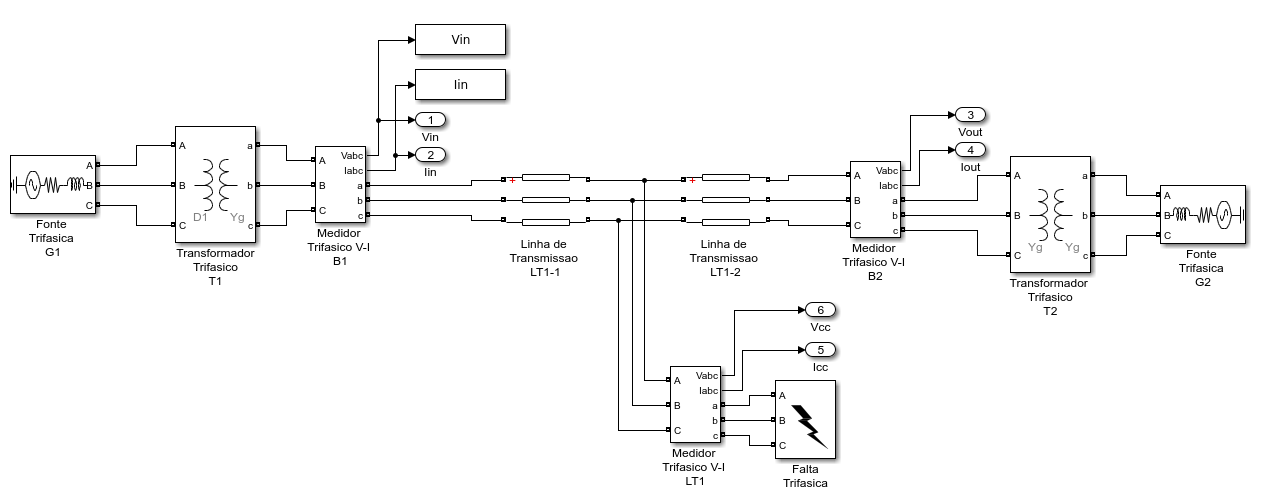
\includegraphics[width=\textwidth]{figuras/modelo_simulink.png}

  \legend{Fonte: Autoria própria.}
\end{figure}

Todos os testes descritos neste trabalho foram realizados considerando a condição de carregamento de 1 SIL, isto é, a potência natural da linha utilizada como referência operacional do sistema. Essa condição foi adotada para estabelecer um ponto nominal comum entre os ensaios, permitindo que as alterações realizadas para validar cada função de proteção fossem controladas em torno de uma mesma base de operação.

Os parâmetros elétricos da linha de transmissão utilizada no modelo são apresentados na Tabela \ref{tab:parametros-linha}. A linha possui tensão nominal de \SI{500}{\kilo\volt} e comprimento de \SI{190}{\kilo\metre}, sendo representada por parâmetros de sequência homopolar e não homopolar.

\begin{table}[H]
  \centering
  \small
  \caption{Parâmetros elétricos da linha de transmissão de \SI{500}{\kilo\volt} e \SI{190}{\kilo\metre}}
  \label{tab:parametros-linha}
  \begin{tabular}{lccc}
    \toprule
    Componente & Resistência & Reatância indutiva & Susceptância \\
    \midrule
    Homopolar & \SI{0,4352}{\ohm\per\kilo\metre} & \SI{1,4427}{\ohm\per\kilo\metre} & \SI{3,5227}{\micro\siemens\per\kilo\metre} \\
    Não homopolar & \SI{0,0161}{\ohm\per\kilo\metre} & \SI{0,2739}{\ohm\per\kilo\metre} & \SI{6,0417}{\micro\siemens\per\kilo\metre} \\
    \bottomrule
  \end{tabular}
  \legend{Fonte: Sistema teste utilizado nas simulações.}
\end{table}

Os dados do gerador equivalente utilizado na condição de 1 SIL são apresentados na Tabela \ref{tab:parametros-gerador}. Esses parâmetros definem a potência de referência, a tensão interna e a impedância associada à fonte do sistema.

\begin{table}[H]
  \centering
  \small
  \caption{Parâmetros do gerador equivalente para a condição de 1 SIL}
  \label{tab:parametros-gerador}
  \begin{tabular}{lcccc}
    \toprule
    Equipamento & Potência & Tensão & Reatância & Resistência \\
    \midrule
    Gerador G1 & \SI{1417,5}{\mega\volt\ampere} & $\SI{15,37}{\kilo\volt}\angle \ang{3,41}$ & \SI{0,04317}{\ohm} & \SI{0,001257}{\ohm} \\
    \bottomrule
  \end{tabular}
  \legend{Fonte: Sistema teste utilizado nas simulações.}
\end{table}

A Tabela \ref{tab:parametros-fonte-equivalente} apresenta os parâmetros da fonte equivalente associada ao terminal remoto do sistema. Foram considerados os parâmetros de 1 SIL, incluindo os valores de tensão e impedâncias equivalentes de Thévenin.

\begin{table}[H]
  \centering
  \small
  \caption{Parâmetros da fonte equivalente para a condição de 1 SIL}
  \label{tab:parametros-fonte-equivalente}
  \begin{tabular}{lccccc}
    \toprule
    Equipamento & Tensão & $R_{1vth}$ & $X_{1vth}$ & $R_{0vth}$ & $X_{0vth}$ \\
    \midrule
    Vth fraca & $\SI{501,27}{\kilo\volt}\angle \ang{-15,97}$ & \SI{7,6980}{\ohm} & \SI{46,188}{\ohm} & \SI{46,188}{\ohm} & \SI{230,9401}{\ohm} \\
    Vth forte & $\SI{498,70}{\kilo\volt}\angle \ang{-6,51}$ & \SI{1,9245}{\ohm} & \SI{11,5475}{\ohm} & \SI{11,5475}{\ohm} & \SI{57,7349}{\ohm} \\
    \bottomrule
  \end{tabular}
  \legend{Fonte: Sistema teste utilizado nas simulações.}
\end{table}

Os transformadores T1 e T2 foram modelados com enrolamentos em conexão $\Delta$/$Y_g$ e $Y_g$/$Y_g$, respectivamente. Os parâmetros elétricos utilizados na representação dos transformadores são apresentados na Tabela \ref{tab:parametros-transformador}.

\begin{table}[H]
  \centering
  \small
  \caption{Parâmetros dos transformadores utilizados no modelo}
  \label{tab:parametros-transformador}
  \begin{tabular}{lc}
    \toprule
    Parâmetro & Valor \\
    \midrule
    Reatância de dispersão do primário (\SI{15}{\kilo\volt}) & \SI{0,0846}{\ohm} \\
    Reatância de dispersão do secundário (\SI{525}{\kilo\volt}) & \SI{31,3380}{\ohm} \\
    Resistência do enrolamento do primário (\SI{15}{\kilo\volt}) & \SI{0,0030}{\ohm} \\
    Resistência do enrolamento do secundário (\SI{525}{\kilo\volt}) & \SI{0,7950}{\ohm} \\
    \bottomrule
  \end{tabular}
  \legend{Fonte: Sistema teste utilizado nas simulações.}
\end{table}

Durante a simulação, são definidos o instante de aplicação da falta, a duração do evento, a frequência nominal, a taxa de amostragem e os canais medidos. As amostras geradas pelo Simulink são enviadas ao workspace do Matlab. A partir desse ponto, os vetores de tempo, tensão e corrente passam a compor a base de dados que será convertida para oscilografia. Essa etapa é importante porque preserva a relação temporal entre os sinais, permitindo que a reprodução física posterior mantenha coerência com o evento simulado.

\begin{figure}[H]
  \centering
  \caption{Amostras simuladas de tensão e corrente}
  \label{fig:amostras-simulink}

  \fbox{\parbox{0.85\textwidth}{\centering Espaço reservado para gráfico das formas de onda simuladas de tensão e corrente antes, durante e após a falta.}}

  \legend{Fonte: Autoria própria.}
\end{figure}

\subsection{Cenários de validação das funções de proteção}

As simulações não foram utilizadas apenas para gerar uma única condição de curto-circuito, mas para construir cenários específicos de validação para cada função de proteção. Dessa forma, os parâmetros do sistema foram alterados de maneira controlada para produzir condições compatíveis com os ajustes definidos no relé emulado.

Para a validação das funções de subtensão e sobretensão, a saída do transformador T1 foi ajustada propositalmente para que a tensão medida no ponto de interesse ficasse abaixo ou acima dos limites configurados na proteção. Assim, foi possível verificar se a função ANSI 27 atuava quando a tensão permanecia inferior ao valor de pickup e se a função ANSI 59 atuava quando a tensão ultrapassava o limite superior configurado.

Para a validação da função de sobrecorrente, a relação de impedância entre os trechos LT1-1 e LT1-2 foi alterada de forma a modificar a corrente observada durante a falta. Ao reduzir ou aumentar a impedância equivalente vista pelo ponto de falta, a corrente de curto-circuito também se altera, permitindo testar diferentes valores de pickup das funções ANSI 50 e ANSI 51.

Para a validação da função de distância, foram simuladas condições nas quais a impedância aparente vista pelo ponto de medição permanecesse dentro ou fora das zonas configuradas. Essa avaliação é feita a partir da relação entre os fasores de tensão e corrente medidos, permitindo verificar a atuação das zonas da função ANSI 21 de acordo com o alcance configurado para a linha.

Por fim, para a função direcional, a validação foi realizada por meio da alteração do ângulo entre as fontes G1 e G2. Essa alteração modifica o sentido do fluxo de potência no sistema, permitindo criar condições de fluxo direto ou reverso. Dessa forma, a função ANSI 67 pôde ser avaliada quanto à capacidade de permitir ou bloquear a atuação da proteção conforme a direção estimada da falta.

A estratégia de ensaio adotada para cada proteção é resumida na Tabela \ref{tab:cenarios-protecao}.

\begin{table}[H]
  \centering
  \small
  \caption{Cenários simulados para validação das funções de proteção}
  \label{tab:cenarios-protecao}
  \begin{tabular}{lll}
    \toprule
    Função & Parâmetro alterado na simulação & Objetivo do ensaio \\
    \midrule
    27 & Tensão na saída de T1 & Produzir tensão abaixo do pickup \\
    59 & Tensão na saída de T1 & Produzir tensão acima do pickup \\
    50/51 & Impedância entre LT1-1 e LT1-2 & Variar corrente de curto-circuito \\
    21 & Impedância aparente vista pelo relé & Testar atuação por zonas \\
    67 & Ângulo entre G1 e G2 & Alterar sentido do fluxo de potência \\
    \bottomrule
  \end{tabular}
  \legend{Fonte: Autoria própria.}
\end{table}

\section{Conversão das amostras para COMTRADE}

Após a simulação, as amostras são processadas pelo script \texttt{comtrade\_generator.m}. Esse script organiza os dados provenientes do Matlab e gera os arquivos do registro COMTRADE, principalmente o arquivo de configuração \texttt{.cfg} e o arquivo de dados correspondente.

O arquivo \texttt{.cfg} contém informações necessárias para interpretação do registro, como identificação do ensaio, frequência nominal, taxa de amostragem, número de canais, unidades e fatores de escala. O arquivo de dados contém os valores amostrados ao longo do tempo. Esse formato é importante porque aproxima o projeto de uma prática real de análise de faltas, visto que o COMTRADE é amplamente utilizado em estudos de oscilografias e eventos em sistemas elétricos de potência \cite{ieee_comtrade,iec_60255_24_2013}.

Do ponto de vista metodológico, essa etapa transforma uma simulação computacional em um registro padronizado. Assim, a plataforma deixa de depender apenas do ambiente Simulink e passa a operar a partir de um formato que pode ser reaproveitado, validado e futuramente substituído por registros de outras origens.

\begin{figure}[H]
  \centering
  \fbox{\parbox{0.85\textwidth}{\centering Espaço reservado para imagem ou captura dos arquivos COMTRADE gerados, destacando os arquivos \texttt{.cfg} e \texttt{.dat}/\texttt{.bdat}.}}
  \caption{Arquivos COMTRADE gerados a partir das amostras simuladas}
  \label{fig:arquivos-comtrade}
\end{figure}

\section{Validação e preparação dos arquivos}

Antes de enviar os arquivos à ESP32 geradora, é necessário verificar se o registro é compatível com a plataforma. Essa validação busca evitar que arquivos incompletos, com canais incompatíveis ou taxas de amostragem inadequadas sejam utilizados nos ensaios.

Os principais critérios considerados são:

\begin{itemize}
  \item existência dos arquivos de configuração e dados;
  \item presença dos canais analógicos necessários;
  \item identificação de um canal de tensão e um canal de corrente;
  \item taxa de amostragem compatível com a reprodução;
  \item quantidade de amostras compatível com a memória disponível;
  \item formato dos dados aceito pela versão embarcada do gerador.
\end{itemize}

Na versão atual do projeto, o script \texttt{run\_embedded\_generator.py} atua como interface de upload e controle da ESP32 geradora. Diferentemente das primeiras versões, nas quais o computador realizava maior parte do tratamento das amostras, a versão atual transfere o processamento principal para a ESP32. Assim, o computador envia os arquivos e a placa realiza localmente a interpretação, escala e preparação dos quadros de reprodução.

\begin{figure}[H]
  \centering
  \fbox{\parbox{0.85\textwidth}{\centering Espaço reservado para captura da etapa de validação/preparação dos arquivos ou tela do terminal antes do envio à ESP32 geradora.}}
  \caption{Validação e preparação dos arquivos para reprodução}
  \label{fig:validacao-arquivos}
\end{figure}

\section{Envio dos dados para a ESP32 geradora}

O envio dos arquivos ocorre por comunicação USB/serial. O script \texttt{run\_embedded\_generator.py} abre a porta serial da ESP32 geradora, aguarda a mensagem de prontidão da placa, envia o arquivo \texttt{.cfg} e o arquivo de dados em blocos e verifica as confirmações de recebimento.

Após o upload, o script solicita o processamento local do registro. A ESP32 geradora interpreta o arquivo de configuração, identifica os canais, calcula os parâmetros de escala e organiza as amostras em estruturas internas de reprodução. Ao final desse processamento, a placa informa que está pronta para reproduzir o evento.

Além disso, o processo gera um arquivo de configuração auxiliar para a ESP32 receptora. Esse arquivo contém informações como escala dos canais, frequência de referência, taxa de amostragem recomendada, valores nominais e mapeamento dos canais de aquisição. Essa etapa é importante para que a recepção interprete corretamente os sinais reproduzidos pela unidade geradora.

\begin{figure}[H]
  \centering
  \fbox{\parbox{0.85\textwidth}{\centering Espaço reservado para captura do terminal durante o upload dos arquivos e confirmação \texttt{READY\_PLAYBACK} da ESP32 geradora.}}
  \caption{Envio dos arquivos COMTRADE para a ESP32 geradora}
  \label{fig:upload-esp32-geradora}
\end{figure}

\section{Reprodução dos sinais na ESP32 geradora}

A ESP32 geradora utiliza o firmware \path{embedded_generator.ino}. Esse firmware é responsável por armazenar os arquivos recebidos, processar o COMTRADE, construir os quadros de reprodução e comandar o DAC MCP4728. O conversor digital-analógico possui resolução de 12 bits e quatro canais, sendo utilizado para reproduzir os sinais de tensão e corrente em forma analógica \cite{microchip_mcp4728}.

Como o DAC trabalha em uma faixa positiva de tensão, os sinais alternados são reproduzidos com um deslocamento em torno de uma tensão média. Dessa forma, uma senoide que originalmente teria valores positivos e negativos é mapeada para uma faixa compatível com o hardware. A Figura \ref{fig:geracao-sinais} ilustra a lógica de reprodução.

\begin{figure}[H]
  \centering
  \begin{tikzpicture}[
    node distance=1.0cm,
    bloco/.style={draw, rounded corners, align=center, minimum width=3.2cm, minimum height=1.0cm, font=\small},
    seta/.style={-{Latex[length=2.5mm]}, thick}
  ]
    \node[bloco] (cfg) {COMTRADE\\\texttt{.cfg} + dados};
    \node[bloco, right=of cfg] (proc) {Processamento\\na ESP32};
    \node[bloco, right=of proc] (frames) {Quadros\\$dt$, $V_{DAC}$, $I_{DAC}$};
    \node[bloco, below=of frames] (dac) {MCP4728\\conversão D/A};
    \node[bloco, left=of dac] (out) {Saídas analógicas\\tensão e corrente};

    \draw[seta] (cfg) -- (proc);
    \draw[seta] (proc) -- (frames);
    \draw[seta] (frames) -- (dac);
    \draw[seta] (dac) -- (out);
  \end{tikzpicture}
  \caption{Etapas de preparação e reprodução dos sinais na ESP32 geradora}
  \label{fig:geracao-sinais}
\end{figure}

O firmware permite diferentes modos de reprodução. O modo de teste gera uma senoide para verificação da bancada. O modo de pré-falta reproduz continuamente os ciclos anteriores ao evento, permitindo estabilizar a recepção antes da falta. O modo de reprodução completa executa o registro COMTRADE, incluindo o período pré-falta, o instante da falta e o comportamento posterior. Esses modos tornam o ensaio repetível e facilitam a visualização do comportamento da proteção.

\begin{figure}[H]
  \centering
  \fbox{\parbox{0.85\textwidth}{\centering Espaço reservado para foto da ESP32 geradora conectada ao DAC MCP4728.}}
  \caption{Unidade embarcada de geração dos sinais}
  \label{fig:unidade-geradora}
\end{figure}

\begin{figure}[H]
  \centering
  \fbox{\parbox{0.85\textwidth}{\centering Espaço reservado para imagem do sinal analógico reproduzido, obtida por osciloscópio, captura ADC ou gráfico de validação.}}
  \caption{Sinais analógicos de tensão e corrente reproduzidos pelo DAC}
  \label{fig:sinais-reproduzidos}
\end{figure}

\section{Aquisição dos sinais na ESP32 receptora}

Os sinais analógicos reproduzidos pelo DAC são aplicados às entradas analógicas da ESP32 receptora. Essa unidade utiliza o firmware \path{embedded_receiver.ino}, responsável por realizar a aquisição dos canais de tensão e corrente, remover o nível médio dos sinais, aplicar os fatores de escala e organizar as amostras para processamento.

A recepção é configurada por meio do script \texttt{run\_embedded\_receiver.py}. Esse script envia à ESP32 receptora os parâmetros necessários para o ensaio, incluindo taxa de amostragem, escalas, valores nominais, frequência de referência e ajustes das funções de proteção. Depois da configuração, a aquisição e a análise são executadas de forma embarcada.

A Figura \ref{fig:recepcao-protecao} apresenta a sequência funcional da unidade receptora.

\begin{figure}[H]
  \centering
  \begin{tikzpicture}[
    node distance=0.9cm,
    bloco/.style={draw, rounded corners, align=center, minimum width=2.8cm, minimum height=0.95cm, font=\small},
    seta/.style={-{Latex[length=2.5mm]}, thick}
  ]
    \node[bloco] (adc) {ADC\\ESP32};
    \node[bloco, right=of adc] (escala) {Offset e\\escala};
    \node[bloco, right=of escala] (ciclo) {Detecção\\de ciclo};
    \node[bloco, below=of ciclo] (fourier) {Fourier\\fasores};
    \node[bloco, left=of fourier] (reles) {Funções\\de proteção};
    \node[bloco, left=of reles] (leds) {LEDs/saídas\\digitais};

    \draw[seta] (adc) -- (escala);
    \draw[seta] (escala) -- (ciclo);
    \draw[seta] (ciclo) -- (fourier);
    \draw[seta] (fourier) -- (reles);
    \draw[seta] (reles) -- (leds);
  \end{tikzpicture}
  \caption{Fluxo de aquisição, processamento e atuação na ESP32 receptora}
  \label{fig:recepcao-protecao}
\end{figure}

\begin{figure}[H]
  \centering
  \fbox{\parbox{0.85\textwidth}{\centering Espaço reservado para foto da ESP32 receptora conectada aos canais analógicos e aos indicadores de atuação.}}
  \caption{Unidade embarcada de recepção e proteção}
  \label{fig:unidade-receptora}
\end{figure}

\section{Processamento das amostras recebidas}

Após a aquisição, as amostras são convertidas para grandezas de engenharia. Como os sinais reproduzidos pelo DAC são deslocados para uma faixa positiva de tensão, a primeira etapa consiste em estimar e remover o offset. Em seguida, aplica-se a escala calculada a partir do registro COMTRADE para recuperar a correspondência entre o sinal de bancada e a grandeza elétrica simulada.

O firmware organiza as amostras por ciclos elétricos. A cada ciclo, são estimadas grandezas como tensão fundamental, corrente fundamental, magnitude dos fasores, ângulo entre tensão e corrente, frequência estimada e indicadores de qualidade da aquisição. A Transformada de Fourier é utilizada porque permite obter magnitude e fase da componente fundamental, informações necessárias para funções como direcional e distância.

Esse processamento cria a ponte entre a forma de onda recebida e a decisão de proteção. Em outras palavras, a ESP32 receptora deixa de trabalhar apenas com valores instantâneos de ADC e passa a operar com grandezas elétricas equivalentes às utilizadas por relés digitais.

\begin{figure}[H]
  \centering
  \fbox{\parbox{0.85\textwidth}{\centering Espaço reservado para gráfico ou captura das grandezas processadas: tensão fundamental, corrente fundamental, fasores, impedância aparente ou eventos calculados.}}
  \caption{Processamento das amostras adquiridas pela ESP32 receptora}
  \label{fig:processamento-receptor}
\end{figure}

\section{Configuração das funções de proteção}

As funções de proteção são configuradas antes do início da aquisição. Essa configuração é realizada por comandos enviados pelo script \texttt{run\_embedded\_receiver.py}, permitindo habilitar ou desabilitar funções e definir os parâmetros de atuação. Essa característica aproxima a plataforma da lógica de ajuste de um relé real.

As principais funções previstas na plataforma são:

\begin{itemize}
  \item subtensão, função ANSI 27, ajustada por percentual de tensão e tempo de atuação;
  \item sobretensão, função ANSI 59, ajustada por percentual de tensão e tempo de atuação;
  \item sobrecorrente instantânea e temporizada, funções ANSI 50 e 51, ajustadas por pickup e atraso;
  \item direcional de sobrecorrente, função ANSI 67, ajustada por sentido, ângulo e janela angular;
  \item distância, função ANSI 21, ajustada por impedância da linha, alcance das zonas e temporização.
\end{itemize}

No caso de falta trifásica, a análise das funções de sobrecorrente e distância torna-se especialmente relevante. A sobrecorrente responde à elevação da corrente durante a falta, enquanto a distância avalia a impedância aparente calculada pela relação entre os fasores de tensão e corrente. A função direcional pode ser associada à função de distância para permitir ou bloquear a atuação, demonstrando a interação entre funções de proteção.

\begin{figure}[H]
  \centering
  \fbox{\parbox{0.85\textwidth}{\centering Espaço reservado para captura do terminal com os comandos de configuração das funções de proteção.}}
  \caption{Configuração das funções de proteção por comandos}
  \label{fig:configuracao-protecoes}
\end{figure}

\section{Lógica de atuação e indicação por LEDs}

A atuação das proteções ocorre quando as grandezas calculadas satisfazem os critérios configurados. Para proteções temporizadas, além da condição elétrica, é necessário que o tempo ajustado seja cumprido. Quando uma função atua, a ESP32 receptora registra o evento e mantém o estado de trip até que seja enviado um comando de reset ou que a placa seja reiniciada.

No projeto, a indicação da atuação é feita por mensagens seriais e por saídas digitais conectadas a LEDs ou a um módulo de relés. A versão atual da ESP32 receptora disponibiliza quatro indicações principais associadas à lógica de distância e direcional:

\begin{itemize}
  \item bloqueio da atuação da função de distância pela lógica direcional;
  \item permissão ou habilitação da atuação;
  \item trip da zona 1 da proteção de distância;
  \item trip da zona 2 da proteção de distância.
\end{itemize}

Esses indicadores permitem visualizar fisicamente o resultado dos algoritmos de proteção. Assim, ao reproduzir uma oscilografia de falta, o aluno pode observar não apenas a forma de onda, mas também o comportamento lógico do relé emulado: condição normal, pickup, bloqueio, permissão e trip.

\begin{figure}[H]
  \centering
  \fbox{\parbox{0.85\textwidth}{\centering Espaço reservado para foto dos LEDs ou módulo de relés indicando bloqueio, permissão, zona 1 e zona 2.}}
  \caption{Indicação física da atuação das proteções}
  \label{fig:indicacao-leds}
\end{figure}

\section{Procedimento experimental}

O procedimento experimental segue uma sequência padronizada para garantir repetibilidade dos ensaios. Inicialmente, seleciona-se a oscilografia COMTRADE correspondente à falta a ser analisada. Em seguida, o script \texttt{run\_embedded\_generator.py} envia os arquivos à ESP32 geradora e solicita o processamento local. Após a confirmação de prontidão, a unidade geradora permanece disponível para executar os modos de teste, pré-falta ou reprodução completa.

Na sequência, a ESP32 receptora é configurada por meio do script \texttt{run\_embedded\_receiver.py}. São definidos os parâmetros de escala e os ajustes das funções de proteção que serão avaliadas no ensaio. Após a configuração, inicia-se a aquisição embarcada.

Com a recepção em execução, a ESP32 geradora reproduz os sinais analógicos de tensão e corrente. Esses sinais são recebidos pela ESP32 receptora, processados por ciclo e avaliados pelos algoritmos de proteção. Durante o ensaio, observam-se os eventos enviados pela serial e os LEDs/saídas digitais correspondentes à atuação das funções.

\begin{figure}[H]
  \centering
  \fbox{\parbox{0.85\textwidth}{\centering Espaço reservado para foto geral da bancada experimental com computador, ESP32 geradora, DAC, ESP32 receptora e LEDs.}}
  \caption{Bancada experimental utilizada nos ensaios}
  \label{fig:bancada-experimental}
\end{figure}

\section{Critérios de avaliação}

A avaliação da plataforma considera critérios funcionais e didáticos. Do ponto de vista funcional, verifica-se se a oscilografia é corretamente convertida, se o COMTRADE é aceito pela plataforma, se a ESP32 geradora reproduz os sinais, se a ESP32 receptora consegue adquirir as amostras e se as funções de proteção atuam de acordo com os parâmetros configurados.

Do ponto de vista didático, avalia-se se o sistema permite acompanhar todo o encadeamento do estudo de proteção: simulação da falta, geração da oscilografia, reprodução física, aquisição, processamento fasorial, decisão do relé e indicação por LEDs. Esse encadeamento é a principal contribuição metodológica da plataforma, pois transforma um conteúdo usualmente teórico em uma experiência prática e observável.

\section{Conclusão}

Este capítulo apresentou a metodologia utilizada no desenvolvimento da plataforma didática. Foram descritas as etapas de simulação, geração de arquivos COMTRADE, validação, envio à ESP32 geradora, reprodução dos sinais pelo DAC MCP4728, aquisição pela ESP32 receptora, processamento fasorial, configuração das funções de proteção e indicação da atuação por LEDs ou saídas digitais.

A metodologia proposta permite integrar ferramentas computacionais e hardware embarcado em um fluxo experimental único. Essa integração possibilita que eventos simulados em sistemas elétricos de potência sejam reproduzidos em bancada e analisados por algoritmos de proteção, estabelecendo a base para a implementação detalhada apresentada no capítulo seguinte.
